\documentclass[a4paper,utf8]{article}
\usepackage{graphicx}
\usepackage[heading,fancyhdr]{ctex}
\usepackage{amsmath,amssymb,geometry,ulem}
\usepackage{array,tabularx,tabulary,mhchem,xspace}
\usepackage{floatrow,subfig,multirow,bigstrut}
\usepackage{siunitx,booktabs,longtable,nameref}
\lineskiplimit=1pt
\lineskip=3pt
\geometry{
    top=25.4mm, 
    left=25mm, 
    right=25mm, 
    bottom=25mm,
    headsep=5.9mm,
}
\ctexset{
    chapter = {
        name = {实验,},
        beforeskip = {-23pt}
    }
}
\newcommand{\fgref}[1]{图~\ref{#1}\xspace}
\newcommand{\seqref}[1]{式~(\ref{#1})}
\newcommand{\expinfo}[6][无]{
    {\zihao{-3}\bfseries\songti
    实验名称:\uline{\hfill\mbox{#2}\hfill} \\[2.9mm]
    学\quad 号:\uline{\makebox[25mm]{#3}}\hfill
    姓\quad 名:\uline{\makebox[25mm]{#4}}\hfill
    班\quad 级:\uline{\makebox[25mm]{#5}} \\[2.9mm]
    合作者:\uline{\makebox[25mm]{#1}} \hfill
    桌\quad 号:\uline{\makebox[25mm]{}}\hfill\makebox[25mm+4em]{}\\[2.9mm]
    指导教师:\uline{\makebox[30mm]{#6}}\hfill\mbox{} \\[2.9mm]
    实验日期:\uline{\makebox[30mm]{}}\hfill\mbox{} \\[58.7mm]
    }
}%\expinfo[合作者]{实验名称}{学号}{姓名}{班级}{指导教师}
\newcommand{\pointingbox}{
    {\zihao{4}\bfseries\songti%
    实验考核\\[3mm]
    \extrarowheight=3mm
    \begin{tabularx}{150mm}{|X|X|X|X|X|}\hline
        \hfil 项目 \hfil  & \hfil 实验预习 \hfil & \hfil 实验过程 \hfil & \hfil 分析与讨论 \hfil & \hfil 总评 \hfil \\[3mm] \hline
        \hfil 评价 \hfil &  &  &  &  \\[3mm] \hline
    \end{tabularx}
    }
}
\newcommand{\derivative}[2]{\frac{\mathrm{d} #1}{\mathrm{d} #2}}
\newcommand{\thinking}[2]{\textbf{#1}\\
答:\begin{minipage}[t]{0.85\textwidth}
    #2
\end{minipage}}

\pagestyle{fancy}
\fancyhf{}
%\fancyhead[C]{材料科学基础实验}
%\fancyfoot[C]{\thepage}
\fancyhead[EC]{\leftmark} \fancyhead[OC]{\rightmark}
\fancyhead[EL,OR]{\thepage}
\fancypagestyle{plain}{\renewcommand{\headrulewidth}{0pt}\fancyhf{}}

\newcounter{Rownumber}
\newcommand*{\Rown}{\stepcounter{Rownumber}\theRownumber}
\newcounter{sample}
\newcommand*{\Sam}{\stepcounter{sample}\thesample}
\newcounter{Fignumber}
\newcommand*{\Fign}{\stepcounter{Fignumber}\theFignumber}

\newcommand*{\resetRown}{\setcounter{Rownumber}{0}}
\newcommand{\qrange}[3]{\qtyrange[range-phrase = \text{$\sim$},range-units =single]{#1}{#2}{#3}}
\floatsetup[table]{capposition=top}
\newcolumntype{C}{>{\hfil}X<{\hfil}}
\renewcommand{\Nameref}[1]{\textbf{\ref{#1}~\nameref{#1}}}
\newcommand{\TTR}[0]{\watt\per\m\per\K} %导入导言
\begin{document}
\begin{center}
    {\mbox{}\\[7em]\zihao{2}\bfseries\songti%
    材料科学基础实验报告}\\[34mm]
    \expinfo{超声波无损探伤实验}{22301077}{张蕴东}{22高分子}{李继玲}
    {\zihao{4}\bfseries\songti
    实验考核\\[3mm]
    \extrarowheight=3mm
    \begin{tabularx}{150mm}{|X|X|X|X|X|}\hline
        \hfil 项目 \hfil  & \hfil 实验预习 \hfil & \hfil 实验过程 \hfil & \hfil 分析与讨论 \hfil & \hfil 总评 \hfil \\[3mm] \hline
        \hfil 评价 \hfil &  &  &  &  \\[3mm] \hline
    \end{tabularx}
    }
\end{center}\newpage
\section{实验目的}
    \begin{itemize}
        \item 学习超声波的产生原理及特点,了解超声波探伤仪的工作原理及使用方法 
        \item 学习超声探头指向性原理及其实际应用
        \item 认识超声换能器及超声波探头的不同种类
        \item 了解超声波的传播、波型和波型转换原理及超声波声速的测量方法
    \end{itemize}
\section{实验原理}%简单描述,含必要的公式和附图;
    超声波是频率高于 20kHz 的机械波,具有穿透力强、传播方向性好等特点,实验所用探头通过压电晶片的逆压电效应,将电能转为机械能以产生脉冲超声波。超声波探头结构复杂,包括压电晶片、保护膜、匹配电感等部分,根据不同结构和应用情况可分为直探头、斜探头和可变角探头。超声波的指向性是指探头发射的声束扩散角大小,与波长、频率及探头内压电晶片尺寸有关。声束扩散角越小,指向性越好,测量精度越高。指向性大小可用公式表示:
    \begin{equation}
        \theta=2\sin^{-1}\left(1.22\frac\lambda D\right)
    \end{equation}\par
    超声波根据波形可分为超声纵波、超声横波和超声表面波三种,在介质界面发生反射、折射和波形转换时需满足斯特令定律:
    \begin{equation}
        \begin{aligned}
            \text{反射:}\frac{\sin\alpha}C&=\frac{\sin\alpha_L}{C_{1L}}=\frac{\sin\alpha_S}{C_{1S}}\\
            \text{折射:}\frac{\sin\alpha}C&=\frac{\sin\beta_L}{C_{2L}}=\frac{\sin\beta_S}{C_{2S}}
        \end{aligned}
    \end{equation}\par
    测量超声波声速可采用直接或相对测量法。直接测量法利用超声波探头内部延迟时间和探头测量的人工反射体回波时间计算声速;相对测量法则通过测量两次反射回波的时间差来计算声速。
\section{实验仪器}%规格及参数
    JDUT-2 型超声波试验仪、DS1102E 双通示波器(100MHz)、直探头、斜探头、CSK-IB 试块、耦合剂(水)等。
\section{实验过程}%简述主要过程和实验内容
    \begin{enumerate}
        \item 组装实验仪器;
        \item 利用直探头测量脉冲超声纵波频率和波长
        \item 测量直探头延迟和间接测量法测量试块纵波声速
        \item 测量斜探头延迟、入射点和间接测量法测试块横波声速
        \item 测量斜探头的折射角
        \item 测量直探头和斜探头的声束扩散角
        \item 使用直探头探测缺陷深度
        \item 使用斜探头探测待测试块内部缺陷位置
    \end{enumerate}
\section{实验数据及处理}
    \subsection{实验数据}
        测得的实验数据见下表:
        \begin{figure}[!ht]
            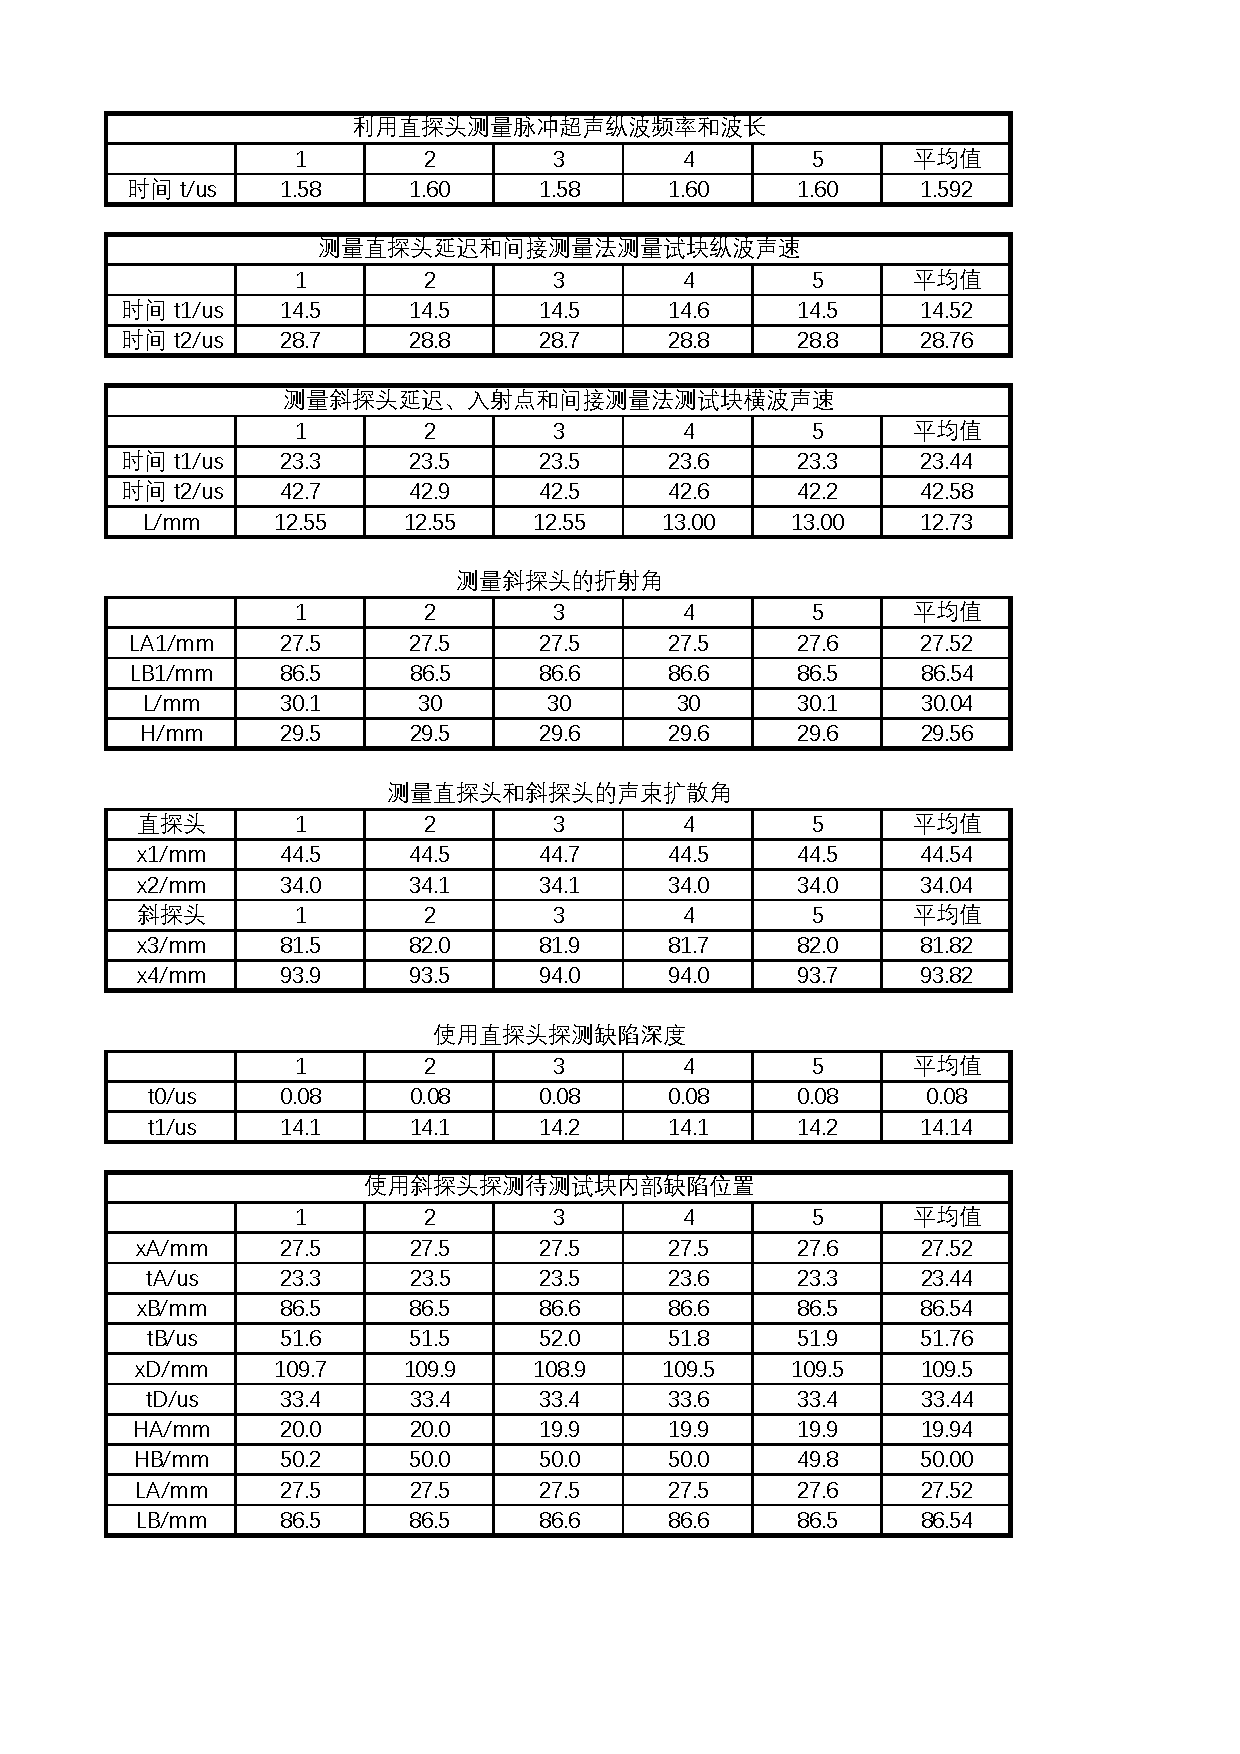
\includegraphics[width=0.8\textwidth]{result.pdf}
        \end{figure}
    \subsection{不确定度分析}
    \subsubsection{A 类不确定度分量的评估}
    对一个随机变量 $x$ 进行了 $n$ 次重复测量,其算术平均值 $\bar{x}$ 作为对被测量 $x$ 的最佳统计评估值,平均值的标准偏差 $s(\bar{x})$ 作为实验结果的标准不确定度,自由度 $\nu=n-1$。计算公式为\\
    \begin{align}
        \bar{x}&=\frac{1}{n}\sum_{i=1}^{n}x_i \label{exp:amean} \\
        s(\bar{x})&=\sqrt{\frac{1}{n(n-1)}\sum_{i=1}^{n}(x_i-\bar{x})^2} \label{exp:astd}
    \end{align}

    \subsubsection{B 类不确定度分量的评估}
    对一个非重复测量得到的量 x 进行不确定度分析时,评估者需根据已获得的信息人为假定其服从某种概率分布来评估其方差 $u^2(x)$ 或标准不确定度 $u(x)$。具体步骤是,首先根据量 $x$ 的变化范围确定其半宽度 $a$,然后根据假定的概率分布计算标准不确定度。\\
    \begin{equation}
        u(x) = \frac a k \label{exp:uncertaintyB}
    \end{equation}
    在 100\% 和 95\% 置信概率下,矩形分布时的包含因子 $k$ 值分别为 $\sqrt{3}$ 和 $1.65$,三角形分布时的包含因子 $k$ 值分别为 $\sqrt{6}$ 和 $1.90$,正态分布时的包含因子 $k$ 值分别为 $3$ 和 $1.96$。

    \subsubsection{直接测量量的合成标准不确定度}
    直接测量量的合成标准不确定度 $u_c(x)$ 由其 A 类标准不确定度分量 $s(\bar{x})$ 与其 B 类标准不确定度分量 $u(x)$ 采用方和根法合成,即\\
    \begin{equation}
        u_c(x) = \sqrt{s^2(\bar{x})+u^2(x)} \label{exp:uncertaintyCombine}
    \end{equation}
    合成标准不确定度 $u_c$ 的自由度称为有效自由度,用 $\nu_\text{eff}$ 表示。当各分量间相互独立且合成量接近正态分布或 t 分布时,有效自由度 $\nu_\text{eff}$ 可以由下面的韦尔奇-萨特韦特(Welch-Satterthwaite)公式计算\\
    \begin{equation}
        \nu_\text{eff}=\frac{u_c^4(x)}{\displaystyle\frac{s^4(x)}{\nu_\text{A}}+\frac{u^4(x)}{\nu_\text{B}}} \label{exp:validFreedom}
    \end{equation}
    式中 $\nu_\text{A}$ 和 $\nu_\text{B}$ 分别是 A 类和 B 类标准不确定度分量对应的自由度数。如果 $\nu_\text{eff}$ 不是整数,则去掉小数部分取整,即将 $\nu_\text{eff}$ 取为一个不大于 $\nu_\text{eff}$ 本身的整数。

    \subsubsection{标准不确定度的传播规律}
    标准不确定度传播规律的数学基础是全微分。假设间接测量量 $y$ 与直接测量量 $x_1$, $x_2$, $x_3$, $\cdots$, $x_n$ 满足函数关系 $y = f(x_1,x_2,x_3,\cdots,x_n)$,且各个直接测量量 $x_1$, $x_2$, $x_3$, $\cdots$, $x_n$ 是相互独立的。对于以标准偏差表示的标准不确定度,需以方和根的形式求和,因此,当各个直接测量量依次有 $u(x_1)$, $u(x_2)$, $u(x_3)$, $\cdots$, $x_n$ 的标准不确定度时,间接测量量 $y$ 的标准不确定度 $u_c(y)$ 可以表示为\\
    \begin{equation}
        u_c^2(y)=\sum_{i=1}^{n}\left[\frac{\partial f}{\partial x_i}\right]^{2}u^2\left(x_{i}\right)=\sum_{i=1}^{n}c_i^2 u^2\left(x_{i}\right) \label{exp:uncertaintyPropagation}
    \end{equation}
    间接测量量 $y$ 的有效自由度由下式计算\\
    \begin{equation}
        \nu_\text{eff}=\frac{u_c^4(y)}{\displaystyle\sum_{i=1}^{n}\frac{c_i u^4(x_i)}{\nu_i}} \label{exp:validFreedom2}
    \end{equation}

    当需要评定扩展不确定度 $U$ 时,可根据合成标准不确定度的有效自由度 $\nu_\text{eff}$ 和给定的置信概率(譬如 95\%),通过查 t 分布表得出包含因子 $k$,进而给出扩展不确定度 $U = k u_c$。

    
    \subsection{实验结果}
        依据以上的公式,下面给出了最终结果及其不确定度:\par
        \subsubsection{直探头延迟、超声波频率和纵波波长、声速的计算}
            \begin{table}[!ht]\caption{计算值}
                \centering\begin{tabular}{c c|c c|c c}\hline
                    $\bar t$ & \SI{1.592}{\us} & $\bar{t_1}$ & \SI{14.52}{\us}& $\bar{t_2}$ & \SI{28.76}{\us} \\ \hline
                    频率 $f$ & \SI{2.512}{\MHz} & 直探头延迟 $t$ & \SI{0.28}{\us}& 纵波声速 $C_L$ & \SI{6.320}{\mm\per\us} \\ \hline
                    纵波波长 $\lambda$ & \SI{2.522}{\mm} &  & & & \\ \hline
                \end{tabular}
            \end{table}\par
            \begin{align*}
                f &= (2.512 \pm 0.027) \unit{\MHz}\\
                t &= (0.28 \pm 0.04) \unit{\us}\\
                C_L &= (6.320 \pm 0.025) \unit{\mm\per\us}\\
                \lambda &= (2.522 \pm 0.026) \unit{\mm}
            \end{align*}
        \subsubsection{斜探头延迟、入射点和横波波长、声速的计算}
            \begin{table}[!ht]\caption{计算值}
                \centering\begin{tabular}{c c|c c|c c}\hline
                    $\bar{t_1}$ & \SI{23.44}{\us} & $\bar{t_2}$ & \SI{42.58}{\us}& $\bar{L}$ & \SI{12.73}{\mm} \\ \hline
                    斜探头延迟 $t$ & \SI{4.30}{\us} & 横波声速 $C_S$ & \SI{3.1348}{\mm\per\us}& 横波波长 $\lambda$ & \SI{1.2476}{\mm} \\ \hline
                     斜探头前沿距离 $L_0$ & \SI{17.27}{\mm} & & & & \\ \hline
                \end{tabular}
            \end{table}\par
            注:在这里只量取了探头到 $R_1$ 的距离,故在实际计算时用 $R_1$ 减去 $\bar{L}$。
            \begin{align*}
                t &= (4.3 \pm 0.2) \unit{\us}\\
                C_S &= (3.14 \pm 0.11) \unit{\mm\per\us}\\
                \lambda &= (1.25 \pm 0.08) \unit{\mm}\\
                L_0 &= (17.27 \pm 0.14) \unit{\mm}
            \end{align*}
        \subsubsection{斜探头的折射角计算}
            \begin{table}[!ht]\caption{计算值}
                \centering\begin{tabular}{c c|c c|c c|c c}\hline
                    $\bar{L_{A1}}$ & \SI{27.52}{\mm} & $\bar{L_{A1}}$ & \SI{86.54}{\mm}& $\bar{L}$ & \SI{30.04}{\mm} & $\bar{H}$ & \SI{29.56}{\mm}\\ \hline
                    \multicolumn{4}{c}{斜探头折射角 $\beta$} & \multicolumn{4}{c}{\SI{44.4325}{\degree}} \\ \hline  
                \end{tabular}
            \end{table}\par
            \begin{align*}
                \beta &= (44.53 \pm 0.37) \unit{\degree}
            \end{align*}
        \subsubsection{直探头和斜探头的声束扩散角的计算}
            \begin{table}[!ht]\caption{计算值}
                \centering\begin{tabular}{c c|c c|c c|c c}\hline
                    $\bar{x_1}$ & \SI{44.54}{\mm} & $\bar{x_2}$ & \SI{34.04}{\mm}& $\bar{x_3}$ & \SI{81.82}{\mm} & $\bar{x_4}$ & \SI{93.82}{\mm}\\ \hline
                    \multicolumn{2}{c}{直探头扩散角 $\theta_1$} & \multicolumn{2}{c}{\SI{15.43}{\degree}} & \multicolumn{2}{c}{斜探头扩散角 $\theta_2$} & \multicolumn{2}{c}{\SI{9.87}{\degree}} \\ \hline
                \end{tabular}
            \end{table}\par
            \begin{align*}
                \theta_1 &= (15.43 \pm 0.56) \unit{\degree}\\
                \theta_2 &= (9.87 \pm 0.11) \unit{\degree}
            \end{align*}
        \subsubsection{直探头探测缺陷深度的计算}
        \begin{table}[!ht]\caption{计算值}
            \centering\begin{tabular}{c c|c c}\hline
                $t_0$ & \SI{0.08}{\us} & $t_c$ & \SI{14.14}{\us}\\ \hline
                \multicolumn{2}{c}{缺陷 C 深度 $H_C$} & \multicolumn{2}{c}{\SI{44.4312}{\mm}} \\ \hline
            \end{tabular}
        \end{table}\par
            \begin{align*}
                H_C &= (44.44 \pm 0.13) ~\unit{\mm}
            \end{align*}
        \subsubsection{待测试块内部缺陷位置的计算}
        \begin{table}[!ht]\caption{计算值}
            \centering\begin{tabular}{c c|c c}\hline
                $t_D$ & \SI{33.44}{\us} & $x_D$ & \SI{109.5}{\mm}\\ \hline
                缺陷 D 深度 $H_D$ & \SI{31.4142}{\mm} & 缺陷 D 水平距离 $L_D$ & \SI{93.6946}{\mm}  \\ \hline
            \end{tabular}
        \end{table}\par
            \begin{align*}
                H_D &= (31.42 \pm 0.027)~\unit{\mm}\\
                L_D &= (93.7 \pm 0.8) ~\unit{\mm}
            \end{align*}
        从上面各个实验与讲义中给出的参考数据的比较可以看出,本次实验除缺陷 D 水平距离的误差较大,其它数据的准确程度和精度都非常可观,说明实验操作较为规范、数据处理五疏漏。值得注意的是本次实验数据均用 Excel 存储,由 Wolfram Mathematica 进行计算和处理,篇幅有限仅展示部分代码作为计算过程参考。
        \begin{figure}[!ht]
            \subfloat[误差计算传递]{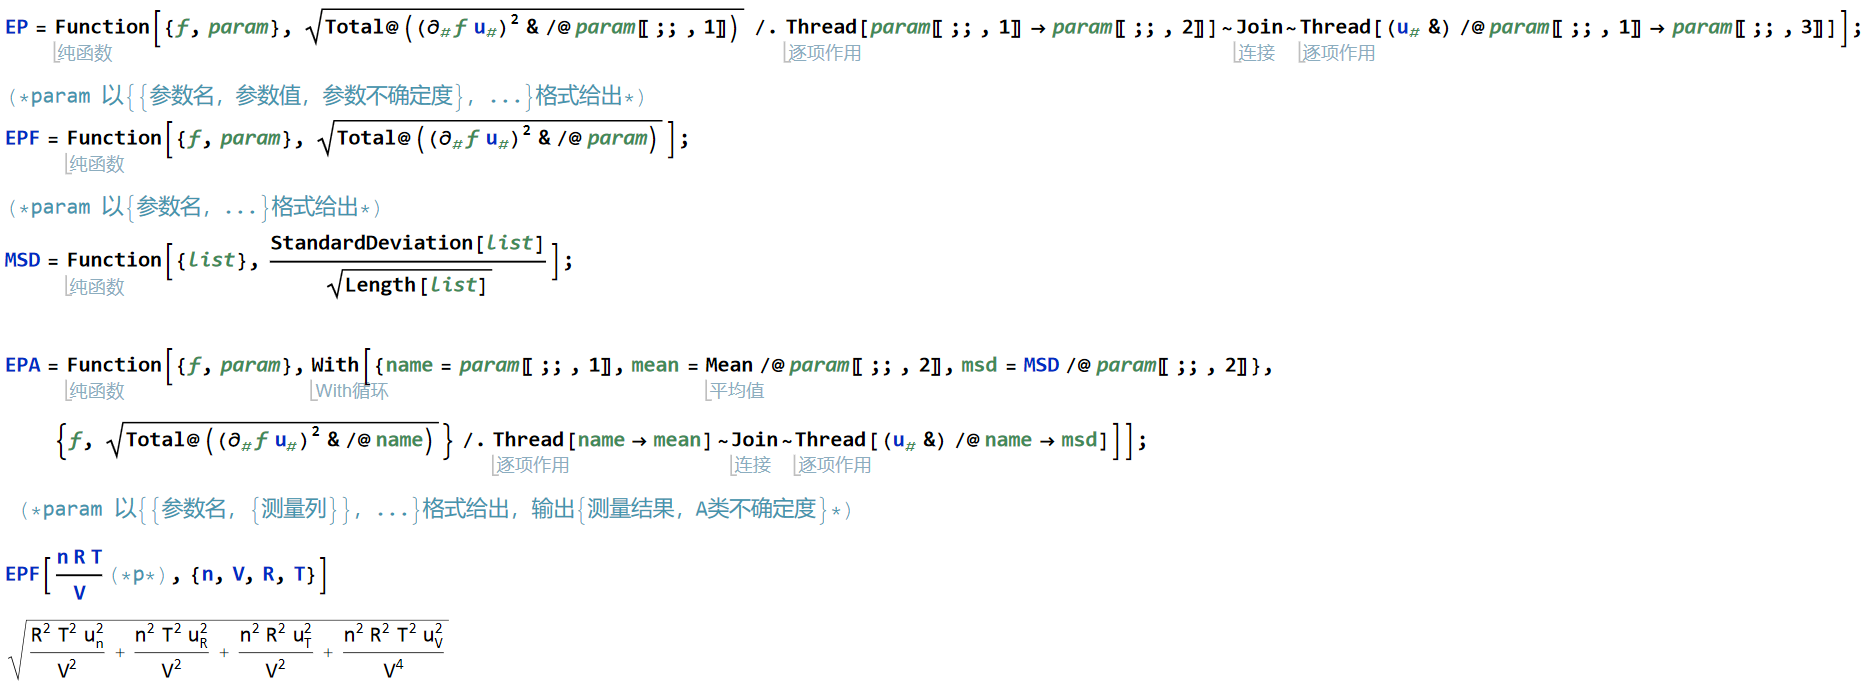
\includegraphics[width=0.4\textwidth]{EP.png}}\\
            \subfloat[公式计算(部分)]{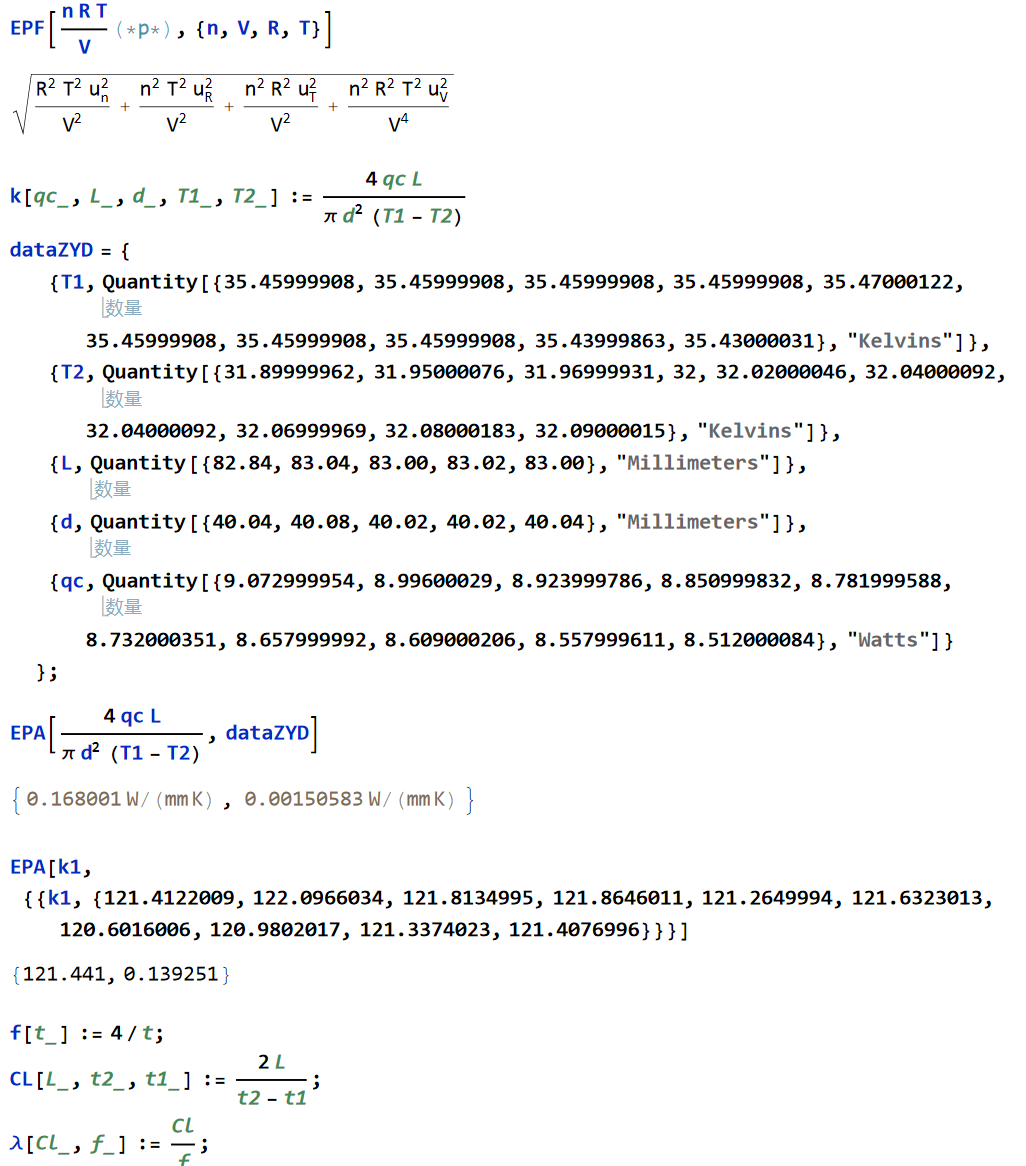
\includegraphics[width=0.4\textwidth]{F.png}}
        \end{figure}
    \subsection{误差分析}
        本次实验主要的误差来源有:
        \begin{itemize}
            \item 系统误差
                \begin{itemize}
                    \item 实验当天的温度、湿度对样品的影响。查阅资料得知,温度、湿度会在一定程度下影响超声波的传播速度,进而影响实验测量。
                    \item 仪器本身精度的影响。刻度尺、示波器和探头所带来的误差。其中,示波器发射和接收器之间可能会有信号衰减和失真,使接收的信号强度降低,影响检测灵敏度和可靠性;也可能会导致信号形状的改变、波形的扭曲或者信号的重叠,影响信号的正确读取和分析。
                    \item 待测样品并非是完全与标准一致的,必然有误差。
                \end{itemize}
            \item 偶然误差
                \begin{itemize}
                    \item 在用刻度尺测量各个长度时,可能会由于估读而产生读取数据的误差。测量声束扩散角的实验中需要找到极大值和振幅减小一半的位置,可能会由于选取示波器上波形的位置而产生主观的读数误差。
                \end{itemize}
        \end{itemize}
        可以通过:根据当天的温度湿度进行结果修正、使用测量精度更高的仪器、多次测量来提高精度
\section{思考题}
    \begin{enumerate}
        \item 测量斜探头延迟和横波声速的时候,为什么斜探头打在圆弧面上,只有超声横波?\par
        超声波的传播受到声阻抗和材料性质的影响。当超声波从一个介质进入另一介质时,根据声阻抗匹配原理,超声波可能会发生折射和反射。斯涅尔定律描述了声波从一个介质传播到另一个介质时发生折射的规律,是光学中折射定律的声学对应。斯涅尔定律指出,对于两个介质界面,入射角(入射声波与法线的夹角)与折射角(折射声波与法线的夹角)的正弦之比,等于两个介质中声速的比值。而当入射角大于第一临界角时,折射角会大于 90 度,这意味着纵波不会进入第二个介质,所以斜探头接收不到超声纵波。
        
        \item 如果将待测试块从铝试块更换为钢试块,对同一斜探头测量到的延迟和入射
        点是否一样?为什么?\par
        一样。延迟本质上是超声波在探头内传播的时间,主要取决于探头本身的特性,入射点也是如此。而在测量时使用的是同一探头,因此延迟和入射点应该是一样的。不同的试样只能缩小或者放大信噪比,改变结果精度。
    \end{enumerate}    
\end{document}